\documentclass{beamer}

\usepackage[czech]{babel}
\usepackage[utf8]{inputenc}
\usepackage{times}
\usepackage[T1]{fontenc}

\mode<presentation>
{
  \usetheme{Warsaw}
  \usecolortheme{crane} 
}

\setbeamertemplate{footline}{
  \leavevmode%
  \hbox{%
  \begin{beamercolorbox}[wd=.333333\paperwidth,ht=2.25ex,dp=1ex,center]{author in head/foot}%
    \usebeamerfont{author in head/foot}\insertshortauthor
  \end{beamercolorbox}%
  \begin{beamercolorbox}[wd=.333333\paperwidth,ht=2.25ex,dp=1ex,center]{title in head/foot}%
    \usebeamerfont{title in head/foot}\insertshortsubtitle
  \end{beamercolorbox}%
  \begin{beamercolorbox}[wd=.333333\paperwidth,ht=2.25ex,dp=1ex,center]{date in head/foot}%
    \usebeamerfont{date in head/foot}\insertframenumber/7
  \end{beamercolorbox}}%
  \vskip0pt%
}

\title{Urychlení metod k-means a mean-shift pomocí 3D akcelerační karty}
\subtitle{Projekt do předmětu GMU (pr05)}
\author[Martin Šimon \& Pavel Širůček]{Martin Šimon \& Pavel Širůček}
\institute{Vysoké učení technické v Brně - Fakulta informačních technologií}
\date{}

\begin{document}

\begin{frame}[plain]
  \titlepage 
\end{frame}
\addtocounter{framenumber}{-1}


\begin{frame}{K-means a mean-shift}
  \begin{itemize}
    \medskip
    \item Metody pro shlukování - použity pro segmentaci obrazu či kvantizaci barev
    \medskip
    \item Paralelizace algoritmů (případně vhodných částí) pro zpracování na GPU
    \medskip
  \end{itemize}
\end{frame}


\begin{frame}{K-means}
  \begin{itemize}
    \item Využito pro kvantizaci barev (3D barevný prostor RGB)
    \medskip
    \item Implementace pomocí 2 kernelů
    \medskip
      \begin{itemize}
        \item První kernel přiřazuje pixely ke středům
        \medskip
        \item Druhý kernel přepočítává středy
        \medskip
      \end{itemize}
    \item Kernely jsou spouštěny tak dlouho, dokud se mění středy
    \medskip
  \end{itemize}
\end{frame}


\begin{frame}{K-means - ukázka výstupu}
  \begin{center}
    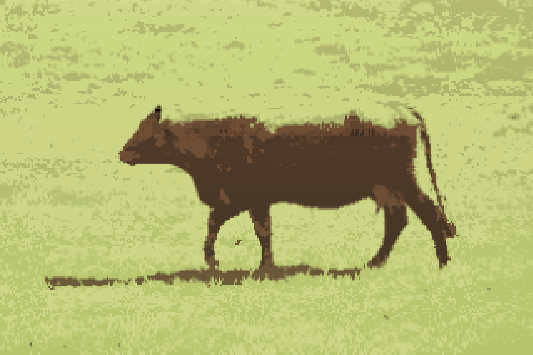
\includegraphics[width=4cm,keepaspectratio]{images/km.pdf}
  \end{center}
\end{frame}


\begin{frame}{Mean-shift}
  \begin{itemize}
    \item Využito pro segmentaci
    \medskip
    \item Vše v jednom kernelu
    \medskip
      \begin{itemize}
        \item
      \end{itemize}
    \medskip
  \end{itemize}
\end{frame}


\begin{frame}{Mean-shift - ukázka výstupu}
  \begin{center}
    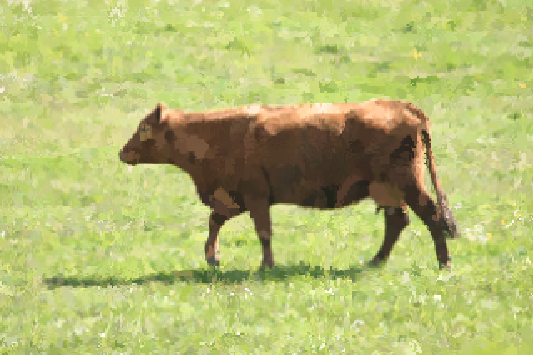
\includegraphics[width=4cm,keepaspectratio]{images/ms.pdf}
  \end{center}
\end{frame}


\begin{frame}{Zrychlení výpočtů}
  \begin{center}
    \begin{tabular}{| c | c | c || c | c | c |}
      \hline
      \multicolumn{3}{| c ||}{K-means} & \multicolumn{3}{ c |}{Mean-shift} \\
      \hline
      CPU & GPU & Akcelerace & CPU & GPU & Akcelerace\\
      \hline
      20ms & ?ms & ?x & 20ms & ?ms & ?x\\
      \hline
    \end{tabular}
  \end{center}
\end{frame}


\begin{frame}{Zdroje}
  \begin{itemize}
    \item 2. cvičení GMU
    \item k-means clustering [http://en.wikipedia.org/wiki/K-means\_clustering]
    \item Meanshift [http://en.wikipedia.org/wiki/Mean-shift]
  \end{itemize}
\end{frame}

\end{document}
